% no answer key
% \documentclass[letterpaper]{exam}

% answer key
\documentclass[letterpaper, landscape]{exam}
\usepackage{2in1, lscape} 
\printanswers

\usepackage{units} 
\usepackage{xfrac} 
\usepackage[fleqn]{amsmath}
\usepackage{float}
\usepackage{mdwlist}
\usepackage{booktabs}
\usepackage{cancel}
\usepackage{polynom}
\usepackage{caption}
\usepackage{fullpage}
\usepackage{comment}
\usepackage{enumerate}
\usepackage{graphicx}

\usepackage{mathtools} 

\newcommand{\dg}{\ensuremath{^\circ}} 
\newcommand{\sgn}{\operatorname{sgn}}

\everymath{\displaystyle}
\title{Calculus I \\ Homework Fifteen \\ Section 3.7}
\author{}
\date{\today}

\begin{document}

  \maketitle

  \section{Homework}
    \begin{itemize*}
      \item read Section 3.7
      \item exercises: 5-11, 13, 15, 18, 20, 23, 24, 29, 31
    \end{itemize*}

  \ifprintanswers

  \section{Solutions}

  \begin{description}

    \item[5] 
      \begin{enumerate}[(a)]
        \item The particle is speeding up between 0 and 1 seconds and slowing down after 
          $t = \unit[1]{s}$.

        \item The particle is slowing down between 0 and 1 seconds and after 2 seconds and speeding
          up between 1 and 2 seconds.

      \end{enumerate}

    \item[6] 
      \begin{enumerate}[(a)]
        \item The particle is slowing down between 0 and 2 seconds and speeding up after 
          $t = \unit[2]{s}$.

        \item The particle is traveling at a roughly constant velocity between 0 and 2 seconds and
          speeding up after that.

      \end{enumerate}

    \item[7]
      \begin{enumerate}[(a)]
        \item 
          \begin{align*}
            v(t)          & = 3t^2 - 9t - 7 \\
            \\
            3t^2 - 9t - 7 & = 0 \\
            t             & = \boxed{ \unit[4]{s} } \\
          \end{align*}

        \item
          \begin{align*}
            a(t)   & = 6t - 9 \\
            \\
            6t - 9 & = 0 \\
            t      & = \boxed{ \unit[1.5]{s} } \\
          \end{align*}

          The acceleration is zero when the object has reached the peak of its flight and is
          stopping and turning around.

      \end{enumerate}

    \item[8]
      \begin{enumerate}[(a)]
        \item 
          \begin{align*}
            v(t) & = 6t + 5 \\
            v(2) & = \boxed{ \unit[17]{m} } \\
          \end{align*}

        \item
          \begin{align*}
            6t + 5 & = 35 \\
            t      & = \boxed{ \unit[5]{s} } \\
          \end{align*}
      \end{enumerate}

    \item[9]
      \begin{enumerate}[(a)]
        \item 
          \begin{align*}
            v(t) & = 10 - 1.66t \\
            v(3) & = \boxed{ \unit[5.03]{m} } \\
          \end{align*}

        \item
          \begin{align*}
            10 t - 0.83 t^2     & = 25 \\
            t                   & \approx \{ \unit[3.5403]{s}, \unit[8.5079]{s} \}
            \\
            v(\unit[3.5403]{s}) & \approx \boxed{ \unit[4.123]{m/s} }
          \end{align*}

      \end{enumerate}
      
    \item[10]
      \begin{enumerate}[(a)]
        \item 
          The maximum height occurs when the velocity is zero:
          \begin{align*}
            v(t)             & = 80 - 32t \\
            80 - 32t         & = 0 \\
            t                & = \unit[2.5]{s} \\
            \\
            h(\unit[2.5]{s}) & = \boxed{ \unit[100]{ft} } \\
          \end{align*}

      \end{enumerate}

    \item[11]
      \begin{enumerate}[(a)]
        \item 
          \begin{align*}
            A(x)              & = x^2 \\
            A'(x)             & = 2x \\
            A'(\unit[15]{cm}) & = \unit[\unit[30]{cm^2/cm}]{} \\
          \end{align*}

          When the side length is 15 cm, adding a little more to each side will increase the area at
          a rate of $\unit[30]{cm^2/cm}$. For instance, increasing the side length from 15 cm to
          15.1 cm will increase the area from 225 cm to 228.01 cm and 
          \[
            228.01 \approx 225 + 30 \cdot 0.1 
          \]
          
        \item
          \begin{align*}
            A(x)  & = x^2 \\
            A'(x) & = 2x \\
            P(x)  & = 4x \\
          \end{align*}

          Adding $\Delta x$ to each side of the square adds a small strip of area $x \Delta x$.
          Adding two of these results in an area change of approximately $2 x \Delta x$. This
          double counts the small corner of area $(\Delta x)^2$ since it is included in both strips.
          This doesn't matter much if $\Delta x$ is small.

      \end{enumerate}

    \item[13]
      \begin{enumerate}[(a)]
        \item 
          \begin{enumerate}[(i)]
            \item 2 to 3: $15.71$
            \item 2 to 2.5: $14.14$
            \item 2 to 2.1: $12.88$
          \end{enumerate}

        \item 
          \begin{align*}
            A(r)  & = \pi r^2 \\
            A'(r) & = 2 \pi r \\
            A'(2) & = 4 \pi \\
          \end{align*}

        \item Adding $\Delta r$ to the radius adds an almost rectangular strip with area:
          \[
            \Delta A \approx Delta r \cdot 2 \pi r \\
          \]
      \end{enumerate}

    \item[15]
      \begin{align*}
        S(r) &= 4 \pi r^2 \\
        S'(r) &= 8 \pi r \\
        \\
        S'(1) &= \unit[25.13]{ft^2/ft} \\
        S'(2) &= \unit[50.27]{ft^2/ft} \\
        S'(3) &= \unit[75.40]{ft^2/ft} \\
      \end{align*}

      The bigger the baloon gets, the more the surface area increases with each
      small change in the radius.

    \item[18]
      \begin{align*}
        V'(t)  & = 6.25t - 250 \\
        \\
        V'(5)  & = \unit[-218.75]{gal/min} \\
        V'(10) & = \unit[-187.5]{gal/min} \\
        V'(20) & = \unit[-125]{gal/min} \\
        V'(40) & = \unit[0]{gal/min} \\
      \end{align*}

      The water drains out more and more slowly as the tank empties. This is because
      the water pressure decreases as the tank empties.

    \item[20]
      \begin{enumerate}[(a)]
        \item $F'(r) = -\frac{2 G m M}{r^3}$

          The minus sign indicates that the gravity decreases as $r$ increases.

        \item Since we are dealing with the one pair of objects, $GmM$ is a constant.
          \begin{align*}
            k         & = G m M \\
            \\
            -2        & = - \frac{2 k}{20000^3} \\
            k         & = 8 \times 10^{12} \\
            \\
            F'(r)     & = - \frac{1.6 \times 10^{13}}{r^3} \\
            F'(10000) & = \unit[-16]{N/km} \\
          \end{align*}

      \end{enumerate}

    \item[23]
      After $t$ hours, the population is 
      \[
        n = 400 \cdot 3^t 
      \]

      The rate of change is:
      \[
        n'(t) = 400 \ln 3 \cdot 3^t
      \]

      After 2.5 hours:
      \[
        n'(2.5) \approx \unit[6851]{bacteria}
      \]

    \item[24]
      \begin{align*}
        f'(t) &= \frac{0.7abe^{ - 0.7 t}}{\left( 1 + be^{ - 0.7 t} \right)^2}
        \\
        20 &= \frac{a}{1 + b} \\
        12 &= \frac{0.7 ab}{\left( 1 + b \right)^2} \\
        \\
        a &= 140 \\
        b &= 6 \\
        \\
        f(t) &= \frac{140}{1 + 6 e^{-0.7t}} \\
      \end{align*}

      As time goes by, the denominator approachs 1 and the yeast population approaches 140 cells. 
      
      See Figure~\ref{fig:ex24}.

      \begin{figure}[H]
        \centering
        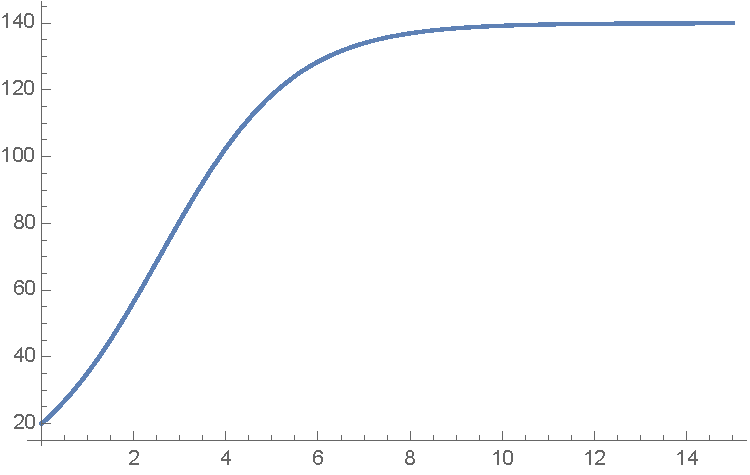
\includegraphics[scale = 0.5]{ex24}
        \caption{Exercise 24}
        \label{fig:ex24}
      \end{figure}


    \item[29]
      \begin{enumerate}[(a)]
        \item 
          \[
            C'(x) = 0.0015x^2 - 0.2x + 12
          \]

        \item $C'(200) = \$32$. This is approximately the cost to produce one
          more item when you are already producing 200 items.

        \item The cost of the 201st item is:
          \[
            C(201) - C(200) \approx \$32.20
          \]
      \end{enumerate}

    \item[31]
      \begin{enumerate}[(a)]
        \item 
          \[
            A'(x) = \frac{p'(x) - p(x)}{x^2} 
          \]

          If $A'(x) > 0$, adding more workers increases the average productivity
          so the company can make more money.

        \item 
          \[
            A'(x) = \frac{p'(x) - p(x)}{x^2} = \frac{p'(x)}{x^2} - \frac{A(x)}{x} \\
          \]

          If $p'(x) > A(x) = \frac{p(x)}{x}$, then
          \begin{align*}
            A'(x) & = \frac{p'(x)}{x^2} - \frac{A(x)}{x} > \frac{A(x)}{x} - \frac{A(x)}{x} = 0 \\
            A'(x) & > 0 \\
          \end{align*}

      \end{enumerate}



    % \item[21]
    %   \begin{enumerate}[(a)]
    %     \item 
    %       \begin{align*}
    %         V             & = \frac{C}{P} \\
    %         \frac{dV}{dP} & = - \frac{C}{P^2} \\
    %       \end{align*}

    %     \item
    %       After 10 minutes, the pressure has increased. The rate of change of
    %       the volume is smaller when the pressure is larger so after 10 minutes
    %       the pressure is increasing at a slower rate.

    %     \item
    %       \begin{align*}
    %         \Beta & = - \frac{1}{V} \cdot \frac{dV}{dP} \\
    %               & = \frac{1}{V} \cdot \cdot \frac{PV}{P} \\
    %               & = \frac{C}{PV} \\
    %       \end{align*}

    %   \end{enumerate}

  \end{description}

  \else
    \vspace{10 cm}
    \begin{quote}
      \begin{em}
        TO DO
      \end{em}
    \end{quote}
    \hspace{2 cm} --TO DO
  \fi

\end{document}

